\section{Literature Review}

The book written by \citeauthor{BookIA} \cite{BookIA} presents all the concepts necessary to start in the field of artificial intelligence (AI).
AI models have been thought of since the early days of computing. It has always been aspired to build an algorithm
that would self-model itself depending on the problem, to have the best possible solution,
and that would be able to increase its own accuracy by simply needing a larger input, without the need to modify
the code itself.

As cited by \citeauthor{AntColonyOptimization} \cite{AntColonyOptimization}, algorithms based on ant colonies
and other insects with similar behaviors began to be thought of in the 1990s.
Noticing details in the way ants organize themselves to find better
paths to achieve their goals, inspired several researchers to design algorithms that imitate it as a way
of optimization for the field of artificial intelligence.

Programming any AI has the problem of always having to worry about the size of the input for training.
An AI that always needs large inputs to get good results needs to make good use of the resources available on the machine.
Therefore, modeling this program taking advantage of parallel computing is essential for good use of these resources.
The performance difference between the sequential version and the parallel version is so significant that designing the algorithms
already thinking about making them parallel can make a big difference \cite{SequentialVSParallel}.

As presented by \citeauthor{ParallelComputingCUDA}, several computational problems can be optimized on GPUs.
The use of CUDA for parallel programming of massive amounts of data becomes extremely necessary, since
Nvidia graphics cards can be up to 250 times faster than a parallel version on Intel CPU \cite{ParallelComputingCUDA}.
Graphics cards have a great capacity to calculate large amounts of data simultaneously and artificial intelligence
is an application that fits perfectly for this purpose.

Many authors like to point out how some programming languages are more efficient than others
when tested on some parameters.
In the article \citetitle{C++vsPython} by \citeauthor{C++vsPython}, it is shown how the difference in the choice of tools
used during the construction of a \emph{software} has a major impact on the final performance of an application as
shown in Figure \ref{fig:comparisonMemorycppvspython}.


\begin{figure}[!ht]
    \centering
    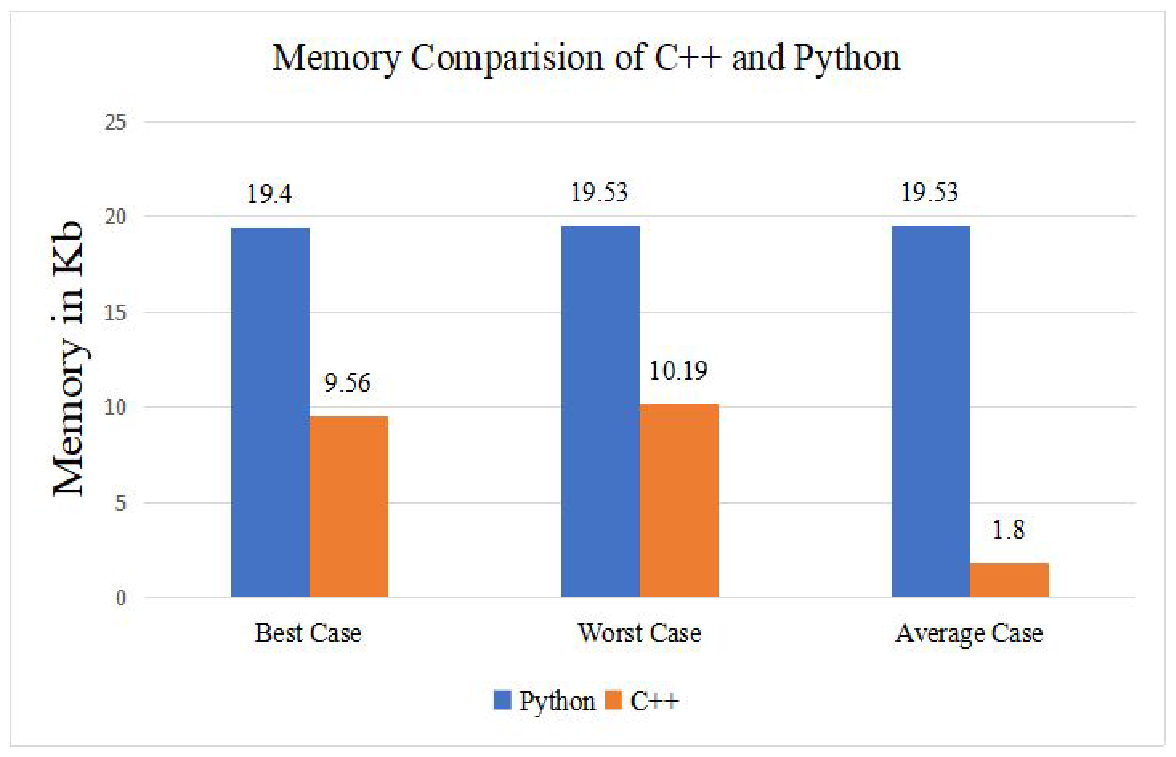
\includegraphics[width=0.5\textwidth]{ComparisonofMemoryConsumptionofSearchingAlgorithm.png}
    \caption[a]{Comparison of memory usage in a search algorithm\footnotemark.}
    \label{fig:comparisonMemorycppvspython}
\end{figure}

\footnotetext{Taken from the article: \citetitle{C++vsPython}.}

Memory usage is extremely important to consider when it comes to AI training context. Runtime is also of paramount importance to calculate since we will always have large inputs to work with. The difference in performance between both languages can be seen in Figure \ref{fig:speedcppvspython}.

\begin{figure}[!ht]
    \centering
    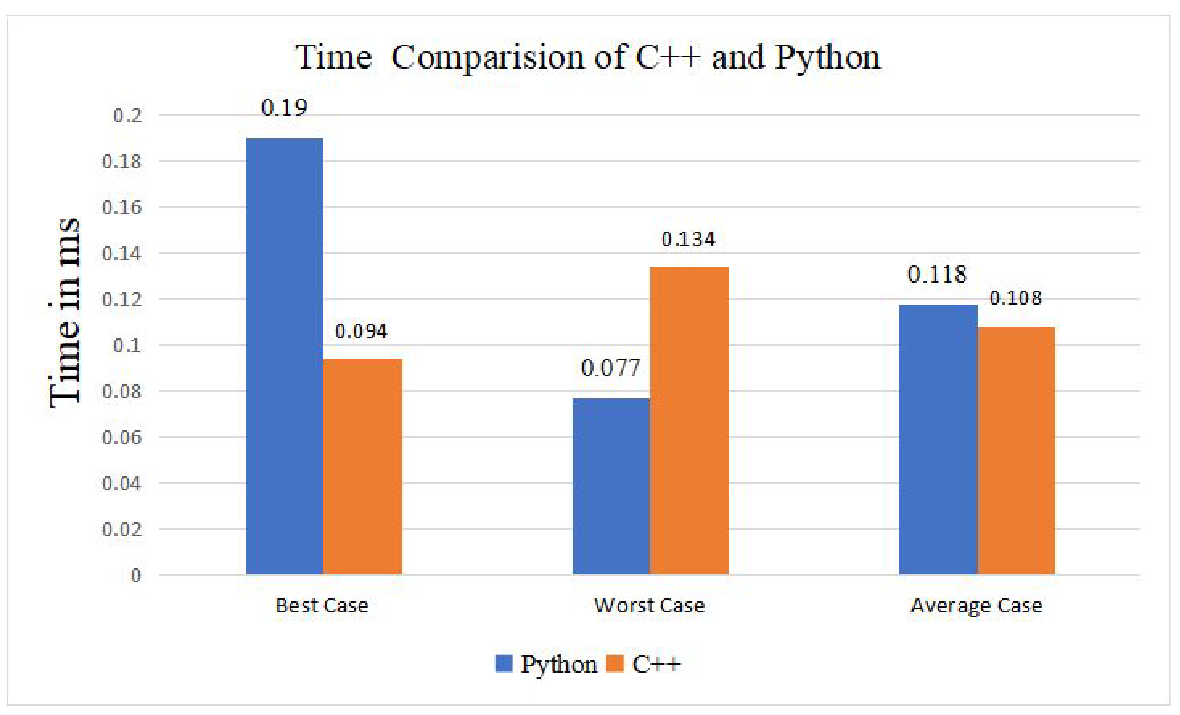
\includegraphics[width=0.5\textwidth]{ComparisonofTimeUtilizationofSearchingAlgorithm.png}
    \caption[a]{Comparison of the execution time of a sequentially executed search algorithm\footnotemark.}
    \label{fig:speedcppvspython}
\end{figure}

\footnotetext{Taken from the article: \citetitle{C++vsPython}.}

It is noticeable that the Python programming language lags behind the C++ language in these measured parameters. The former is considerably simpler to use and teach to new programmers \cite{C++vsPython}. With this in mind, researcher \citeauthor{HPC_Python} presented in his article \citetitle{HPC_Python} how Python became the favorite language for teachers to teach and its immense versatility in the scientific field. Due to its ease of use, there was a lot of community attention to improving the performance of this language until it became competitive with C++.

Efforts were made to increase its efficiency, as mentioned by \citeauthor{JIT}, who in his work for IBM as early as 2007, was thinking about how to improve the performance of the Java programming language using a Just-in-Time Compiler. This feature allows a language to be compiled into Bytecode, which is equivalent to an intermediate programming language between what the machine can understand and what the programmer actually wrote. This allowed a code not to be fully compiled for a specific processor architecture but to be modified at the time of execution to the most efficient machine assembly code available \cite{JIT}.


Considering that Python is an interpreted language. Combining the idea of \emph{JIT} that had been used for several years in the Python interpreter could yield good results. The first test conducted by \citeauthor{NumbaLLVMJIT} yielded excellent results, as shown in Figure \ref{fig:numbavspythonsequencial}.

\begin{figure}[!ht]
    \centering
    \begin{tabular}{|c|c|c|}
        \hline
        Matrix Size & Numba & C \\
        \hline
        64 x 64 & 463x & 453x \\
        \hline
        128 x 128 & 454x & 407x \\
        \hline
        256 x 256 & 280x & 263x \\
        \hline
        512 x 512 & 276x & 268x \\
        \hline
    \end{tabular}
    \caption[a]{Comparison between the execution time of Numba and a C code for matrix multiplication\footnotemark[3].}
    \label{fig:numbavspythonsequencial}
\end{figure}

% Appears at the bottom of the page, not related to the text being written around it
\footnotetext[3]{Taken from the article: \citetitle{NumbaLLVMJIT}.}

With these results, it is possible to demonstrate that with the right optimizations, Python can be made as performant as C++. Many other optimizations were made to achieve even better performance, such as deferred loop specialization, rewriting of matrix equations, and the use of tools for generating optimized bytecode with LLVM.

Algorithms for selecting the best instance, like the \emph{K-Means}, have always been a reference when discussing clustering algorithms. In the article written by \citeauthor{KmeansAlgorithm} \cite{KmeansAlgorithm}, it is shown how there are several extremely efficient implementations for this algorithm and how the complexity order can be elevated, as shown in Figure \ref{fig:complexitykmeans}.

\begin{figure}[!ht]
    \centering
    \begin{tabular}{|c|c|c|c|}
        \hline
        Complexity & \emph{K-Means} & \emph{Constrained-K-Means} & \emph{X-Means} \\
        \hline
        Time & $O(n^2)$ & $O(kn)$ & $O(n\log k_{max})$ \\
        \hline
        Space & $O((n+k)d)$ & $O((n+k)d)$ & $O((n+k)d)$ \\
        \hline
    \end{tabular}
    \caption[a]{Complexity of some \emph{K-Means} implementations\footnotemark.}
    \label{fig:complexitykmeans}
\end{figure}

\footnotetext{Taken from the article: \citetitle{KmeansAlgorithm}.}
